\documentclass[11pt,conference,compsocconf]{IEEEtran}
\usepackage{tikz}
\usepackage{amsmath}
\usepackage{amssymb}
\usepackage{amsthm}
\usepackage{bm}
\usepackage[linesnumbered]{algorithm2e}
\makeatletter
\renewcommand{\@algocf@capt@plain}{above}
\makeatother
\usepackage[colorlinks,urlcolor=blue,citecolor=hotpink,linkcolor=blue]{hyperref}
\usetikzlibrary{decorations.pathreplacing}
\usetikzlibrary{arrows}
\usetikzlibrary{snakes}
\usetikzlibrary{calc}
\let\emptyset\varnothing
\definecolor{hotpink}{rgb}{0.9,0,0.5}
\definecolor{deepgray}{gray}{0.35}
\definecolor{deepgray2}{gray}{0.25}
\definecolor{deepgray3}{gray}{0.10}
\definecolor{lightgray}{gray}{0.95}
\definecolor{lightgray2}{gray}{0.85}
\definecolor{purple1}{RGB}{239,229,244}
\definecolor{purple2}{RGB}{216,191,216}
\definecolor{lightblue}{rgb}{0.73,0.33,0.83}
\definecolor{lightpurple}{rgb}{.8,.2,.8}
\definecolor{textcolor}{rgb}{0,0,5}
\definecolor{blue1}{RGB}{187,217,238}
\definecolor{blue2}{RGB}{235,244,250}
\definecolor{yellow1}{RGB}{255,255,102}
\definecolor{blue3}{RGB}{63,40,96}
\definecolor{red1}{RGB}{255, 102, 102}
\definecolor{green1}{RGB}{102, 255, 102}
\newtheorem{lemma}{Lemma}
\newtheorem{thm}{Theorem}
\newtheorem{defn}{Definition}
\theoremstyle{definition}
\def\proof{\par{\bf Proof}. \ignorespaces}
\def\qedsymbol{\vbox{\hrule\hbox{%
                     \vrule height1.3ex\hskip0.8ex\vrule}\hrule}}
\def\endproof{\qquad\qedsymbol\medskip\par}

% Some very useful LaTeX packages include:
% (uncomment the ones you want to load)


% *** MISC UTILITY PACKAGES ***
%
%\usepackage{ifpdf}
% Heiko Oberdiek's ifpdf.sty is very useful if you need conditional
% compilation based on whether the output is pdf or dvi.
% usage:
% \ifpdf
%   % pdf code
% \else
%   % dvi code
% \fi
% The latest version of ifpdf.sty can be obtained from:
% http://www.ctan.org/tex-archive/macros/latex/contrib/oberdiek/
% Also, note that IEEEtran.cls V1.7 and later provides a builtin
% \ifCLASSINFOpdf conditional that works the same way.
% When switching from latex to pdflatex and vice-versa, the compiler may
% have to be run twice to clear warning/error messages.

% *** CITATION PACKAGES ***
%
\usepackage{cite}
% cite.sty was written by Donald Arseneau
% V1.6 and later of IEEEtran pre-defines the format of the cite.sty package
% \cite{} output to follow that of IEEE. Loading the cite package will
% result in citation numbers being automatically sorted and properly
% "compressed/ranged". e.g., [1], [9], [2], [7], [5], [6] without using
% cite.sty will become [1], [2], [5]--[7], [9] using cite.sty. cite.sty's
% \cite will automatically add leading space, if needed. Use cite.sty's
% noadjust option (cite.sty V3.8 and later) if you want to turn this off.
% cite.sty is already installed on most LaTeX systems. Be sure and use
% version 4.0 (2003-05-27) and later if using hyperref.sty. cite.sty does
% not currently provide for hyperlinked citations.
% The latest version can be obtained at:
% http://www.ctan.org/tex-archive/macros/latex/contrib/cite/
% The documentation is contained in the cite.sty file itself.

% *** GRAPHICS RELATED PACKAGES ***
%
\ifCLASSINFOpdf
  % \usepackage[pdftex]{graphicx}
  % declare the path(s) where your graphic files are
  % \graphicspath{{../pdf/}{../jpeg/}}
  % and their extensions so you won't have to specify these with
  % every instance of \includegraphics
  % \DeclareGraphicsExtensions{.pdf,.jpeg,.png}
\else
  % or other class option (dvipsone, dvipdf, if not using dvips). graphicx
  % will default to the driver specified in the system graphics.cfg if no
  % driver is specified.
  % \usepackage[dvips]{graphicx}
  % declare the path(s) where your graphic files are
  % \graphicspath{{../eps/}}
  % and their extensions so you won't have to specify these with
  % every instance of \includegraphics
  % \DeclareGraphicsExtensions{.eps}
\fi

\usepackage{url}
% correct bad hyphenation here
\hyphenation{op-tical net-works semi-conduc-tor}


\begin{document}
%
% paper title
% can use linebreaks \\ within to get better formatting as desired
\title{Breadth First Searches Over Evolving Graphs}

% author names and affiliations
% use a multiple column layout for up to two different
% affiliations
% \and

\author{
\IEEEauthorblockN{Jiahao Chen}
\IEEEauthorblockA{Computer Science and Artificial Intelligence Laboratory,\\
Massachusetts Institute of Technology,\\
Cambridge, Massachusetts, 02139-4307, USA\\
jiahao@mit.edu}
\and
\IEEEauthorblockN{Weijian Zhang}
\IEEEauthorblockA{School of Mathematics,\\
University of Manchester,\\
Manchester, M13 9PL, England, UK\\
weijian.zhang@manchester.ac.uk}
}

\maketitle

\begin{abstract}
We present a generalization of the breadth first search (BFS) algorithm on
evolving graphs and prove its correctness. The BFS generates paths with nontrivial
structure, which we term temporal paths. We also show with simple counterexamples
that simple products of adjacency matrices do not have the correct combinatorial
properties of enumerating temporal paths. On the contrary, the correct generalization
of BFS requires careful tracking of active nodes which participate in the definition
of edges at specific times. We discuss how the structure of temporal paths leads
to nontrivial matrix structure in adjacency matrix representations of evolving
graphs, as well as implications for real world applications
such as the analysis of citation networks.
\end{abstract}

\begin{IEEEkeywords}
~Evolving graph; complex network; breadth first search; data mining.
\end{IEEEkeywords}

% For peer review papers, you can put extra information on the cover
% page as needed:
% \ifCLASSOPTIONpeerreview
%\begin{center} \bfseries EDICS Category: 3-BBND \end{center}
% \fi
%
% For peerreview papers, this IEEEtran command inserts a page break and
% creates the second title. It will be ignored for other modes.
\IEEEpeerreviewmaketitle

\section{Introduction}

Let's imagine a game played by three people, numbered $1$, $2$, and $3$,
each of whom has a message, labeled $a$, $b$, and $c$ respectively.
At each turn, one particular player is allowed to talk to one other player,
who must in turn convey all the messages in his or her possession.
The goal of the game is to collect all the messages.
Suppose $1$ talks to $2$ first, and $2$ in turn talks to $3$.
Then, $3$ can collect all the messages even without talking to $1$ directly.
However, if $2$ talks to $3$ before $1$ talks to $2$, then
$3$ can never get $a$.

We can use analyze the spread of information between the players using graph
theory. In this process, the time ordering of events matters, and hence its
graph representation $G(t) = (V(t), E(t))$ must be time dependent.
Such a graph is called an ``evolving graph''~\cite{fkp89,bkmu12},
``evolving network'' or %XXX WHO?
``time-dependent graph''. %XXX WHO?

Treatments of evolving graphs vary in their generality and focus.
Kivel\"a \textit{et al.}~\cite{kabg14} treats time dependence as a special
case of families of graphs with multiple interrelationships.
Others like Flajolet \textit{et al.}~\cite{fkp89} use time to index the family
of related graphs, but are not concerned with explicit time-dependent processes.
Yet others focus on incremental updates to large graphs~\cite{bkmu12}.
Here, we describe evolving graphs as a time-ordered sequence of graphs, similar
to the study of metrized graphs by Tang and coworkers~\cite{ntmm13,tmml09,tsmm09,tmml10}
the dynamics of communities by Grindrod, Higham and coworkers~\cite{gphe11,grihig13}.

The game described at the beginning can be encoded in terms of analyzing the
microscopic dynamics of an evolving graph. The spread of information to the
winner can be described in terms of discrete paths through the evolving graph,
and can be interpreted naturally as a graph traveral problem. Traversals of an
ordinary (static) graph may be computed using well known methods such as the
breadth-first search (BFS). However, a proper description of the dynamics
requires paths that also move monotonically forward in time, thus necessating
a generalization of the ordinary BFS algorithm.

An informal description of BFS generalized to evolving graphs can be found in
\cite{tmml09}. However, it turns out that the proper generalization involves
paths of nontrivial structure which sometimes contradict na\"ive generalizations
of results derived from static graphs.
In this paper, we present a complete description of the BFS algorithm for evolving graphs.
The algebraic formulation of this algorithm makes explicit several subtleties in the correct
determination of relevant trajectories, which we term \textit{temporal paths},
which in turn can have important consequences for the computation and interpretation
of quantities which can be expressed as sums over paths, e.g.\ Katz centrality.



\section{Breadth-First Search over Evolving Graphs}
\label{sec:breadth-first-search}


\subsection{Temporal Paths over Active Nodes}
\label{sec:temporal-paths}

\begin{figure}[h]
 \begin{center}
    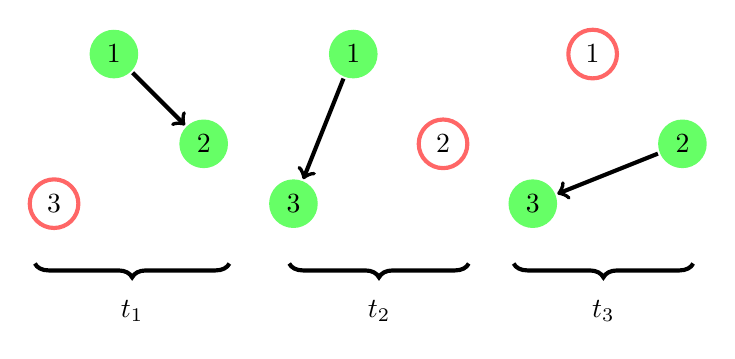
\begin{tikzpicture}[scale=.38, line width =1.5pt]
  \node[circle,fill=green1, minimum size=0.2cm] (n7) at (-5,7) {2};
  \node[circle,draw=red1, minimum size=0.2cm] (n8) at (-10,5) {3};
  \node[circle,fill=green1, minimum size=0.2cm] (n10) at (-8,10) {1};

  \node[circle,draw=red1, minimum size=0.2cm] (n6) at (3,7) {2};
  \node[circle,fill=green1, minimum size=0.2cm] (n4) at (-2,5) {3};
  \node[circle,fill=green1, minimum size=0.2cm] (n1) at (0,10) {1};

   \node[circle,fill=green1, minimum size=0.2cm] (n11) at (11,7) {2};
  \node[circle,fill=green1, minimum size=0.2cm] (n12) at (6,5)  {3};
  \node[circle,draw=red1, minimum size=0.2cm] (n14) at (8,10) {1};

  \foreach \from/\to in {n10/n7, n1/n4, n11/n12}
   \draw[every edge,->] (\from) -- (\to);
\draw [decorate,decoration={brace,amplitude=5pt},xshift=-4pt,yshift=0pt]
(4,3) -- (-2,3) node [midway,yshift=-0.6cm]{ $t_2$};
\draw [decorate,decoration={brace,amplitude=5pt},xshift=-4pt,yshift=0pt]
(-4,3) -- (-10.5,3) node [midway,yshift=-0.6cm]{ $t_1$};
\draw [decorate,decoration={brace,amplitude=5pt},xshift=-4pt,yshift=0pt]
(11.5,3) -- (5.5,3) node [midway,yshift=-0.6cm]{ $t_3$};
    \end{tikzpicture}
\end{center}
\caption{An evolving graph with 3 time stamps $t_1$, $t_2$ and $t_3$.
At each time stamp, the evolving graph is represented as a graph.
The green filled nodes in the figure are active nodes.}
\label{fig:eg_shortest_path}
\end{figure}

The key new idea in generalizing BFS to evolving graphs is to be able to compute
paths that traverse multiple times. We call the relevant paths
\textit{temporal paths}.

Figure~\ref{fig:eg_shortest_path} shows a small example of a evolving
directed graph, $G_3 = \langle G^{[1]}, G^{[2]}, G^{[3]}\rangle$, consisting of
a sequence of three graphs $G^{[i]}$, each bearing a time stamp $t_i$.
There are directed edges $1\rightarrow2$ at time $t_1$,
$1\rightarrow3$ at time $t_2$, and $2\rightarrow3$ at time $t_3$.
Each edge exists only at a particular discrete time and the nodes connected
by edges are considered \textit{active} at that time.

Temporal paths connect only active nodes in ways that respect time ordering.
Thus the sequences
$\langle (1, t_1), (1, t_2), (3, t_2), (3, t_3) \rangle$ and
$\langle (1, t_1), (2, t_1), (2, t_3), (3, t_3) \rangle$
are both examples of \textit{temporal paths} from $(1, t_1)$ to $(3, t_3)$,
which are drawn as dotted lines with arrowheads in Figure~\ref{fig:active}.
However, $\langle (1, t_1), (1, t_2), (2, t_2), (3, t_2), (3, t_3) \rangle$
is not a temporal path because node 2 is inactive at time $t_2$.


\begin{figure}[h]
 \begin{center}
    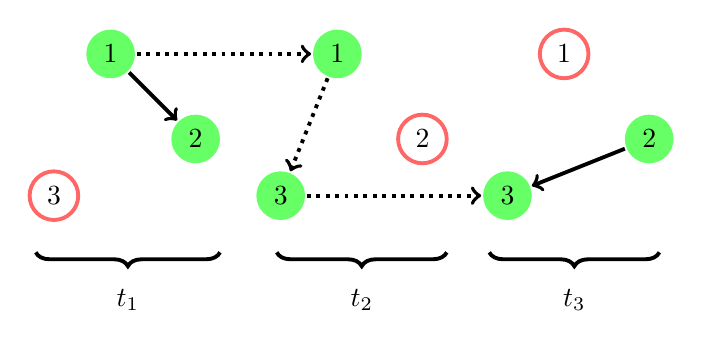
\begin{tikzpicture}[scale=.36, line width =1.4pt]
  \node[circle,fill=green1, minimum size=0.2cm] (n7) at (-5,7) {2};
  \node[circle,draw=red1, minimum size=0.2cm] (n8) at (-10,5) {3};
  \node[circle,fill=green1, minimum size=0.2cm] (n10) at (-8,10) {1};

  \node[circle,draw=red1, minimum size=0.2cm] (n6) at (3,7) {2};
  \node[circle,fill=green1, minimum size=0.2cm] (n4) at (-2,5) {3};
  \node[circle,fill=green1, minimum size=0.2cm] (n1) at (0,10) {1};

   \node[circle,fill=green1, minimum size=0.2cm] (n11) at (11,7) {2};
  \node[circle,fill=green1, minimum size=0.2cm] (n12) at (6,5)  {3};
  \node[circle,draw=red1, minimum size=0.2cm] (n14) at (8,10) {1};

  \foreach \from/\to in {n10/n7, n11/n12}
   \draw[every edge,->] (\from) -- (\to);
     \draw[dotted,->](n1) -- (n4);
  \draw[dotted,->](n10) -- (n1);
  \draw[dotted,->](n4) -- (n12);
\draw [decorate,decoration={brace,amplitude=5pt},xshift=-4pt,yshift=0pt]
(4,3) -- (-2,3) node [midway,yshift=-0.6cm]{ $t_2$};
\draw [decorate,decoration={brace,amplitude=5pt},xshift=-4pt,yshift=0pt]
(-4,3) -- (-10.5,3) node [midway,yshift=-0.6cm]{ $t_1$};
\draw [decorate,decoration={brace,amplitude=5pt},xshift=-4pt,yshift=0pt]
(11.5,3) -- (5.5,3) node [midway,yshift=-0.6cm]{ $t_3$};
    \end{tikzpicture}
   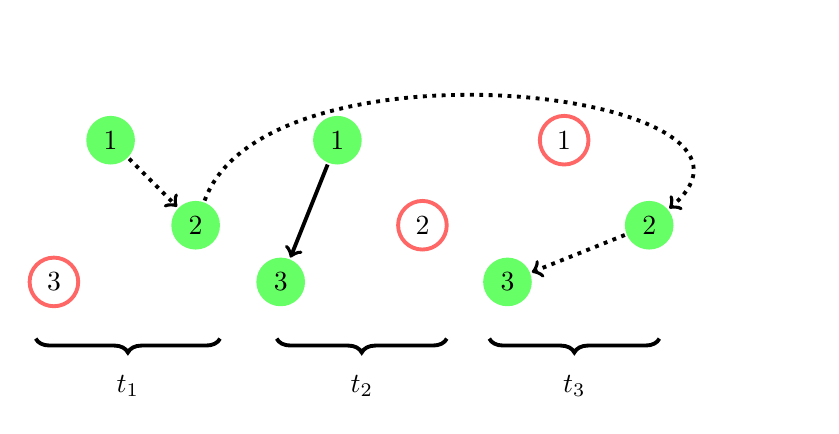
\begin{tikzpicture}[scale=.36, line width =1.4pt]
  \node[circle,fill=green1, minimum size=0.2cm] (n7) at (-5,7) {2};
  \node[circle,draw=red1, minimum size=0.2cm] (n8) at (-10,5) {3};
  \node[circle,fill=green1, minimum size=0.2cm] (n10) at (-8,10) {1};

  \node[circle,draw=red1, minimum size=0.2cm] (n6) at (3,7) {2};
  \node[circle,fill=green1, minimum size=0.2cm] (n4) at (-2,5) {3};
  \node[circle,fill=green1, minimum size=0.2cm] (n1) at (0,10) {1};

   \node[circle,fill=green1, minimum size=0.2cm] (n11) at (11,7) {2};
  \node[circle,fill=green1, minimum size=0.2cm] (n12) at (6,5)  {3};
  \node[circle,draw=red1, minimum size=0.2cm] (n14) at (8,10) {1};

  \foreach \from/\to in {n1/n4}
   \draw[every edge,->] (\from) -- (\to);
     \draw[dotted,->](n7) to[out=70, in=40] (n11);
  \draw[dotted,->](n10) -- (n7);
   \draw[dotted,->](n11) -- (n12);
\draw [decorate,decoration={brace,amplitude=5pt},xshift=-4pt,yshift=0pt]
(4,3) -- (-2,3) node [midway,yshift=-0.6cm]{ $t_2$};
\draw [decorate,decoration={brace,amplitude=5pt},xshift=-4pt,yshift=0pt]
(-4,3) -- (-10.5,3) node [midway,yshift=-0.6cm]{ $t_1$};
\draw [decorate,decoration={brace,amplitude=5pt},xshift=-4pt,yshift=0pt]
(11.5,3) -- (5.5,3) node [midway,yshift=-0.6cm]{ $t_3$};
    \end{tikzpicture}
\end{center}
\caption{An evolving graph with 3 time stamps $t_1$, $t_2$ and $t_3$.
The black dashed lines of the two figures indicate two temporal paths from $(1, t_1)$ to $(3,t_3)$.}
\label{fig:active}
\end{figure}

The restriction that temporal paths may only traverse active nodes reflects
underlying structure in many real world applications, such as analyzing the
influence of nodes over social networks. We will also show later in
Section~\ref{sec:temp-paths-adjac}
that the resulting structure of allowable temporal paths leads to nontrivial
subtleties in the generalization of algorithms and concepts from ordinary
(static) graphs.



\subsection{Breadth-First Traversal Over Temporal Paths}
\label{sec:evolving-graph-bfs}

The example presented above in Section~\ref{sec:temporal-paths}
demonstrates how the notion of active nodes restrict the set of temporal paths
that need to be considered when traversing an evolving graph.

We now give a general description of the BFS algorithm over evolving graphs,
both directed and undirected, which correctly takes into account the structure
of temporal paths.
Our notation generalizes the standard notations for static graphs presented in
\cite{even12,kegi11}.

\begin{defn}
An \textbf{evolving graph} $G_n$ is a sequence of
(static) graphs
$G_n = \langle G^{[1]}, G^{[2]}, \ldots, G^{[n]} \rangle$ with associated
time labels $t_1, t_2, \ldots, t_n$ respectively.
Each $G^{[t]} = (V^{[t]}, E^{[t]})$ represents a (static) graph labeled by a
time $t$.
\end{defn}

Intuitively, an evolving graph is some discretization of the continuous-time family $G(t)$:

\begin{center}
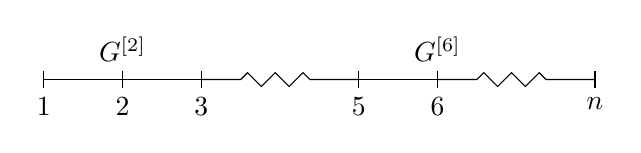
\begin{tikzpicture}[snake=zigzag, line before snake = 5mm, line after snake = 5mm]
    % draw horizontal line
    \draw (0,0) -- (2,0);
    \draw[snake] (2,0) -- (4,0);
    \draw (4,0) -- (5,0);
    \draw[snake] (5,0) -- (7,0);

    % draw vertical lines
    \foreach \x in {0,1,2,4,5,7}
      \draw (\x cm,3pt) -- (\x cm,-3pt);

    % draw nodes
    \draw (0,0) node[below=3pt] {$ 1 $} node[above=3pt] {$   $};
    \draw (1,0) node[below=3pt] {$ 2 $} node[above=3pt] {$ G^{[2]} $};
    \draw (2,0) node[below=3pt] {$ 3 $} node[above=3pt] {$  $};
    \draw (3,0) node[below=3pt] {$  $} node[above=3pt] {$  $};
    \draw (4,0) node[below=3pt] {$ 5 $} node[above=3pt] {$  $};
    \draw (5,0) node[below=3pt] {$ 6 $} node[above=3pt] {$ G^{[6]}$};
    \draw (6,0) node[below=3pt] {$  $} node[above=3pt] {$  $};
    \draw (7,0) node[below=3pt] {$ n $} node[above=3pt] {$ $};
  \end{tikzpicture}
\end{center}


We assume no particular relation between the node and edge sets for each static
graph $G^{[t]} = (V^{[t]}, E^{[t]})$. In particular, we allow the node sets to
change over time, so that each $V^{[t]}$ may be different. Changing
node sets happen naturally in citation networks, where nodes may appear or
disappear from the citation network over time.
The addition, removal, or relabeling of nodes can be expressed in terms
of a map $\Pi^{[t,t^\prime]} : V^{[t]} \rightarrow V^{[t^\prime]}$ that expresses
the appropriate permutations and/or projections.



\begin{defn}
A \textbf{temporal node} is a pair $(v, t)$, where $v\in V^{[t]}$ is a node at
a time $t$.
\end{defn}


\begin{defn}
An \textbf{active node} is a temporal node $(v,t)$ if there exists at least one
edge $e\in E^{[t]}$ that connects $v\in V^{[t]}$ to another node $w\in V^{[t]}$,
$w\ne v$.

An \textbf{inactive node} is a temporal node that is not an active node.
\end{defn}

In Figure~\ref{fig:eg_shortest_path}, the temporal nodes $(1,t_1)$ and $(2,t_2)$
are active nodes, whereas the temporal node $(3,t_1)$ is an inactive node.


\begin{defn}
A \textbf{temporal path} of length $m$ on an evolving graph $G_n$
from temporal node $(v_1, t_1)$ to temporal node $(v_m, t_m)$ is
a time-ordered sequence of active nodes,
$\langle (v_1, t_1), (v_2, t_2), \ldots, (v_m, t_m) \rangle$.
Here, time ordering means that $t_1 \leq t_2 \leq \cdots \leq t_m$ and
$v_i = v_j$ iff $t_i \ne t_j$.
\end{defn}

This definition of a temporal path differs from that of the dynamic walk
in \cite{gphe11,grihig13} in its explicit requirement of containing only active
nodes. The definition implies that if either or both end points of a temporal
path are inactive, then the entire temporal path must be the empty sequence
$\langle \rangle$. Keeping track explicitly of the time labels of each temporal
node allows greater generality to cases where the node sets change over time.
Furthermore, we shall show later in \ref{sec:temp-paths-adjac}
that the explicit bookkeeping of the time labels is essential for correctly
generalizing the BFS to evolving graphs.


The following definition of \textbf{forward neighbors} generalizes the notion of
neighbors and reachability in static graphs.


\begin{defn}
The \textbf{$k$-forward neighbors} of a temporal node $(v, t)$ are the temporal nodes
that are the $k+1$st temporal node in every temporal path of length $k+1$ starting
from $(v, t)$. The \textbf{forward neighbors} of a temporal node $(v, t)$ are its
1-forward neighbors.
\end{defn}

In Figure~\ref{fig:eg_shortest_path},
the forward neighbors of $(1, t_1)$ are $(2, t_1)$ and $(1, t_2)$ and
the forward neighbors of $(2, t_1)$ is $(2, t_3)$.
The 2-forward neighbors of $(1, t_1)$ are
$(2, t_1), (1, t_2), (2, t_2)$ and $(3, t_2)$.
By construction, time stamp of every forward neighbor of an active node $(v, t)$
must be no earlier than $t$.


\begin{defn}
The distance from a temporal node $(v, t)$ to a temporal node $(w, s)$ is
the $k$ for which $(w, s)$ is a $k$-forward neighbor of $(v, t)$.
\end{defn}

Note that this notion of distance is not a metric, since the distance from $(v, t)$
to $(w, s)$ will in general differ from the distance of $(v, t)$ from $(w, s)$
owing to time ordering.


\begin{defn}
A temporal node $(w, s)$ is \textbf{reachable} from a temporal node $(v, t)$ if
the distance to $(w, s)$ from a temporal node $(v, t)$ there exists some finite
integer $k$ for which $(w, s)$ is a $k$-forward neighbor of $(v, t)$.
\end{defn}


The BFS on evolving graphs is described in Algorithm~\ref{alg:bfs}.
Given an evolving graph $G_n$ and a root $(v_1, t_1)$,
Algorithm~\ref{alg:bfs} returns all temporal notes reachable from the root and
their distances from the root.
$reached$ is a dictionary from temporal nodes to integers whose key set represents
all visited temporal nodes and whose value set are the corresponding distances
from the root.

The BFS constructs a tree inductively by discovering all $k$-forward neighbors
of the root before proceeding to all $(k+1)$-forward neighbors of the root.
Within the outermost loop, the algorithm iterates over $frontier$, a list of all
temporal nodes of distance $k$ from the root. The $nextfrontier$ list is populated
with all temporal nodes that are forward neighbors of any temporal node in the
$frontier$ list which have not yet been reached by the algorithm.


\begin{figure}[h]
 \begin{center}
    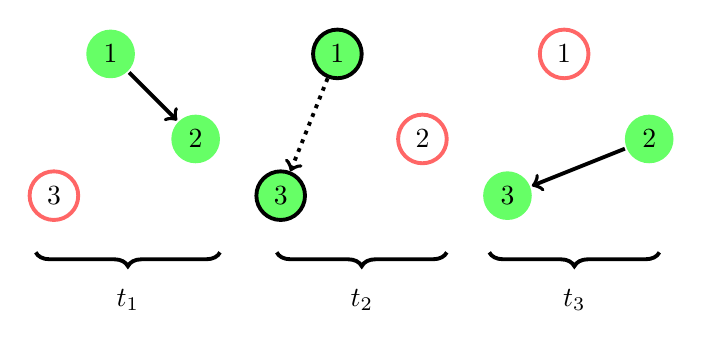
\begin{tikzpicture}[scale=.36, line width =1.4pt]
  \node[circle,fill=green1, minimum size=0.2cm] (n7) at (-5,7) {2};
  \node[circle,draw=red1, minimum size=0.2cm] (n8) at (-10,5) {3};
  \node[circle,fill=green1, minimum size=0.2cm] (n10) at (-8,10) {1};

  \node[circle,draw=red1, minimum size=0.2cm] (n6) at (3,7) {2};
  \node[circle,fill=green1, draw=black, minimum size=0.2cm] (n4) at (-2,5) {3};
  \node[circle,fill=green1, draw=black, minimum size=0.2cm] (n1) at (0,10) {1};

   \node[circle,fill=green1, minimum size=0.2cm] (n11) at (11,7) {2};
  \node[circle,fill=green1, minimum size=0.2cm] (n12) at (6,5)  {3};
  \node[circle,draw=red1, minimum size=0.2cm] (n14) at (8,10) {1};

  \foreach \from/\to in {n10/n7, n11/n12}
   \draw[every edge,->] (\from) -- (\to);
     \draw[dotted,->](n1) -- (n4);
  %\draw[dotted,->](n10) -- (n1);
  %\draw[dotted,->](n4) -- (n12);
\draw [decorate,decoration={brace,amplitude=5pt},xshift=-4pt,yshift=0pt]
(4,3) -- (-2,3) node [midway,yshift=-0.6cm]{ $t_2$};
\draw [decorate,decoration={brace,amplitude=5pt},xshift=-4pt,yshift=0pt]
(-4,3) -- (-10.5,3) node [midway,yshift=-0.6cm]{ $t_1$};
\draw [decorate,decoration={brace,amplitude=5pt},xshift=-4pt,yshift=0pt]
(11.5,3) -- (5.5,3) node [midway,yshift=-0.6cm]{ $t_3$};
    \end{tikzpicture}
   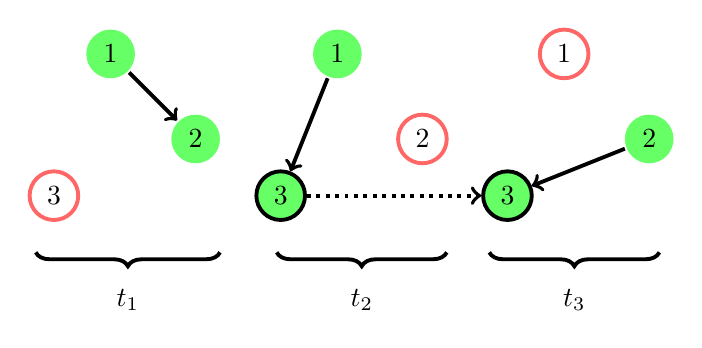
\begin{tikzpicture}[scale=.36, line width =1.4pt]
  \node[circle,fill=green1, minimum size=0.2cm] (n7) at (-5,7) {2};
  \node[circle,draw=red1, minimum size=0.2cm] (n8) at (-10,5) {3};
  \node[circle,fill=green1, minimum size=0.2cm] (n10) at (-8,10) {1};

  \node[circle,draw=red1, minimum size=0.2cm] (n6) at (3,7) {2};
  \node[circle,fill=green1, draw=black, minimum size=0.2cm] (n4) at (-2,5) {3};
  \node[circle,fill=green1, minimum size=0.2cm] (n1) at (0,10) {1};

   \node[circle,fill=green1, minimum size=0.2cm] (n11) at (11,7) {2};
  \node[circle,fill=green1, draw=black, minimum size=0.2cm] (n12) at (6,5)  {3};
  \node[circle,draw=red1, minimum size=0.2cm] (n14) at (8,10) {1};

  \foreach \from/\to in {n1/n4, n10/n7, n11/n12}
   \draw[every edge,->] (\from) -- (\to);
    % \draw[dotted,->](n7) to[out=70, in=40] (n11);
  \draw[dotted,->](n4) -- (n12);
  % \draw[dotted,->](n11) -- (n12);
\draw [decorate,decoration={brace,amplitude=5pt},xshift=-4pt,yshift=0pt]
(4,3) -- (-2,3) node [midway,yshift=-0.6cm]{ $t_2$};
\draw [decorate,decoration={brace,amplitude=5pt},xshift=-4pt,yshift=0pt]
(-4,3) -- (-10.5,3) node [midway,yshift=-0.6cm]{ $t_1$};
\draw [decorate,decoration={brace,amplitude=5pt},xshift=-4pt,yshift=0pt]
(11.5,3) -- (5.5,3) node [midway,yshift=-0.6cm]{ $t_3$};
    \end{tikzpicture}
   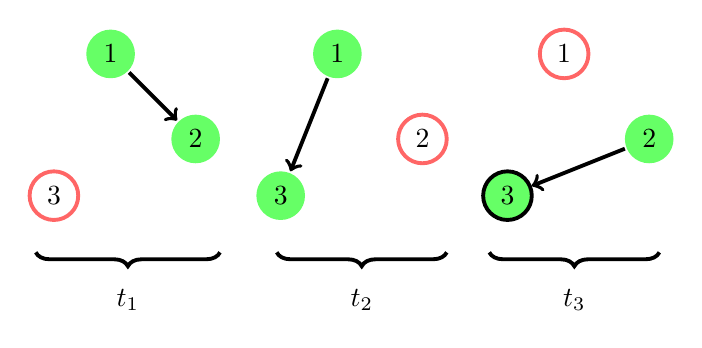
\begin{tikzpicture}[scale=.36, line width =1.4pt]
  \node[circle,fill=green1, minimum size=0.2cm] (n7) at (-5,7) {2};
  \node[circle,draw=red1, minimum size=0.2cm] (n8) at (-10,5) {3};
  \node[circle,fill=green1, minimum size=0.2cm] (n10) at (-8,10) {1};

  \node[circle,draw=red1, minimum size=0.2cm] (n6) at (3,7) {2};
  \node[circle,fill=green1, minimum size=0.2cm] (n4) at (-2,5) {3};
  \node[circle,fill=green1, minimum size=0.2cm] (n1) at (0,10) {1};

   \node[circle,fill=green1, minimum size=0.2cm] (n11) at (11,7) {2};
  \node[circle,fill=green1, draw = black, minimum size=0.2cm] (n12) at (6,5)  {3};
  \node[circle,draw=red1, minimum size=0.2cm] (n14) at (8,10) {1};

  \foreach \from/\to in {n1/n4, n10/n7, n11/n12}
   \draw[every edge,->] (\from) -- (\to);
    % \draw[dotted,->](n7) to[out=70, in=40] (n11);
  %\draw[dotted,->](n10) -- (n7);
   %\draw[dotted,->](n11) -- (n12);
\draw [decorate,decoration={brace,amplitude=5pt},xshift=-4pt,yshift=0pt]
(4,3) -- (-2,3) node [midway,yshift=-0.6cm]{ $t_2$};
\draw [decorate,decoration={brace,amplitude=5pt},xshift=-4pt,yshift=0pt]
(-4,3) -- (-10.5,3) node [midway,yshift=-0.6cm]{ $t_1$};
\draw [decorate,decoration={brace,amplitude=5pt},xshift=-4pt,yshift=0pt]
(11.5,3) -- (5.5,3) node [midway,yshift=-0.6cm]{ $t_3$};
    \end{tikzpicture}
\end{center}
\caption{An evolving graph with 3 time stamps $t_1$, $t_2$ and $t_3$.
The circled green filled nodes indicate a BFS process starting at active node
$(1, t_2)$.}
\label{fig:example}
\end{figure}

As a simple example, consider the BFS on the example graph in
Figure~\ref{fig:eg_shortest_path} starting from the root $(1, t_2)$.
The $frontier$ list is first initialized to $\{(1,t_2)\}$.
Since the only forward neighbor of $(1,t_2)$ is $(3,t_2)$,
iteration $k=1$ produces $reached[(3,t_2)]=1$ and $nextfrontier = \{(3,t_2)\}$.
In the next iteration $k=2$, the only forward neighbor of $(3,t_2)$ is $(3,t_3)$,
so $reached[(3,t_3)]=2$ and $nextfrontier = \{(3,t_3)\}$ and so on.
The algorithm terminates after $k=3$ after verifying that $(3,t_3)$ has no
forward neighbors.

The preceding example illustrates the fact that $G^{[1]}$ plays no part in the
BFS traversal of $G_n$ starting from $(1, t_2)$. In general, all $G^{[t]}$ with
time stamps $t < t'$ for a starting node $(v, t')$ are irrelevant to the BFS
traversal. Hence without loss of generality we may assume that BFS is always
computed with a root at time $t_1$, the earliest time stamp in $G_n$.

\begin{algorithm}[h]
 \SetKwFor{For}{for}{}{end}
 \SetKwFor{While}{while}{}{end}
 \SetKwFor{If}{if}{}{end}
 \SetKwFunction{nei}{forwardneighbors}
 \SetKwProg{Fn}{function}{}{end}
 \Fn{BFS($G_n, (v_1,t_1)$)}{
  $reached[(v_1,t_1)] = 0$ \\
  $frontier = \{(v_1,t_1)\}$ \\
  $k = 1$ \\
  \While{$frontier \ne \emptyset$}{
   $nextfrontier = \emptyset$ \\
   \For{$(v,t) \in frontier$}{
     \For{$(v',t') \in$\nei{$(v,t)$}}{
          \If{$(v',t') \notin d$}{
              $reached[(v',t')] = k$\\
              $nextfrontier = nextfrontier \cup \{(v',t')\}$ \\
              }
         }
       }
  $frontier = nextfrontier$ \\
  $k = k+1$ \\
  }
  \textbf{return} $reached$
}
\caption{Breadth-first search (BFS) on an evolving graph $G_n$ starting from a
root $(v_1, t_1)$. The return value, $reached$, is a dictionary mapping all
reachable temporal notes from the root to their distances from the root. At the
end of each iteration $k$, the $frontier$ set contains all temporal nodes of
distance $k$ from the root.
}
\label{alg:bfs}
\end{algorithm}

\begin{thm}[Correctness of the evolving graph BFS]
Let $G_n$ be an evolving graph and $(v_1, t_1)$ be an active node of $G_n$.
Then Algorithm~\ref{alg:bfs} discovers every active node that is reachable from
the root $(v_1, t_1)$, and $reached[(v, t)]$ is the distance from $(v_1, t_1)$
to $(v, t)$.
\label{thm:correct}
\end{thm}

\IEEEproof
Define the set of temporal nodes
$\tilde V_L^{[t]} = \{(v_1)_t = (v_1, t) | (v_1, v_2) \in E^{[t]}\}$, which
consists of the active nodes at time $t$ which participate on the left side of an edge.
Similarly, $\tilde V_R^{[t]} = \{(v_2)_t = (v_2, t) | (v_1, v_2) \in E^{[t]}\}$
are the corresponding active nodes on the right side of an edge. Then
$\tilde V^{[t]} = \tilde V_L^{[t]} \cup \tilde V_R^{[t]}$ is the set of active
nodes at time $t$, and $V = \bigcup_t \tilde V^{[t]}$ is the set of all
active nodes in $G_n$.

Similarly, define an edge set $E' = \{(u_s,v_t)|u_s=(u,s)\in V,
v_t=(v,t)\in V, v=u, s<t\}$, which consists of temporal nodes that connect
active nodes sharing the same node at different times. Each edge in $E'$ is then
in 1-1 correspondence with a temporal path of length 2,
$\langle (v,s), (v,t) \rangle$.
Define also $\tilde E^{[t]} = \{(e, t)|e\in E^{[t]}\}$, which are simply the edge
sets in $G_n$ with time labels. Then $E = \bigcup_t \tilde E^{[t]} \cup E'$ is
the set of all edges representing all allowed temporal paths of length 2.

The node set $V$ and edge set $E$ now define a static graph $G=(V,E)$ that is in
1-1 correspondence with the evolving graph $G_n$. The node set $V$ of $G$ is in
1-1 correspondence with active nodes of $G_n$ while the edge set $E$ is in 1-1
correspondence with all temporal paths of length 2 on $G_n$.

We now establish a similar 1-1 correspondence of forward neighbors of an active
node with a subset of $G$.
By definition, the forward neighbors of some active node $(v, t) \in G_n$ are
active nodes of either the form $(v, t')$ for some $t' > t$ or $(u, t)$ for some
$u\ne v$. Clearly, the former are elements of $E' \subseteq E$ while the latter
are elements of $E^{[t]} \subseteq \bigcup_s \tilde E^{[s]} \subseteq E$.
Thus each forward neighbor of an active node $(v, t) \in G_n$ is in 1-1
correspondence with a node in $V$ that is a neighbor of $v_t \in V$.

The correctness of BFS on the evolving graph $G_n$ now follows from the
correctness of BFS on the static graph $G$, since we have also established a 1-1
correspondence for every intermediate quantity in Algorithm~\ref{alg:bfs}.
\endproof


As presented, the BFS over evolving graphs makes no assumptions about how the
evolving graph $G_n$ is represented. Suppose it is represented by a collection of
adjacency lists, one for each active node in $G_n$. Then we have that the
asympotic complexity of BFS on $G_n$ is the same as that for BFS on $G$, using
the 1-1 construction of $G$ from $G_n$.

\begin{thm}[Complexity of the evolving graph BFS]
Let $G_n$ be an evolving graph represented using adjacency lists,
$(v_1, t_1)$ be an active node of $G_n$, and $G=(V,E)$ be the static graph
constructed from $G_n$ using the 1-1 correspondences defined in the proof of
Theorem~\ref{thm:correct}. Then the asymptotic complexity of
Algorithm~\ref{alg:bfs} is $O(|E| + |V|)$.
\end{thm}

\IEEEproof
Any edge in any edge set of $G_n$ can be accessed in constant time in random
access memory. By construction, BFS on $G_n$ is in 1-1 correspondence with BFS
on the static graph $G$. The number of operations of BFS on $G$ is $O(|E| + |V|)$,
and so the result follows.
\endproof


\section{Formulating the Evolving Graph BFS with Linear Algebra}
\label{sec:representation}


\subsection{Not All Temporal Paths Can Be Expressed by Products of Adjacency Matrices}
\label{sec:temp-paths-adjac}

For a static graph $G$ with adjacency matrix $A$, $(A^k)_{ij}$ counts the number
of paths of length $k$ between node $i$ and node $j$. Na\"ively, one might want
to generalize this result to evolving graphs by postulating that the $(i,j)$th
entry of the discrete path sum
\begin{align}
S^{[t_n]} = A^{[t_1]}A^{[t_n]} + \sum_{t_1 \le t \le t_n} A^{[t_1]}A^{[t]}A^{[t_n]}
+ \dots \nonumber \\
+ \sum_{t_1 \le t \le t' \le \dots \le t_n}
A^{[t_1]}A^{[t]}A^{[t']}\cdots A^{[t_n]}
\label{eq:sum}
\end{align}
counts the number of temporal paths from $(i,t_1)$ to $(j,t_n)$.
However, this postulate is incorrect.
In the example of Figure~\ref{fig:eg_shortest_path},
\[
(S^{[t_3]})_{13} = \left(A^{[t_1]}A^{[t_2]}A^{[t_3]} + A^{[t_1]}A^{[t_3]}\right)_{13} = 1
\]
even though there are clearly two temporal paths from
$(1, t_1)$ to $(3, t_3)$ as shown in Figure~\ref{fig:active}.
% Indeed, Grindrod et al. \cite{gphe11} observe
% that the $(i,j)$ entry of $A^{[1]}A^{[2]}\cdots A^{[n]}$ counts the number of
% temporal paths of length $n$ from $(i, 1)$ to $(j, n)$, which
% go through exactly one edge at each time stamp between
% $t_1$ and $t_n$.
% Intuitively, it seems that the $(i,j)$ entry of
% the summation of all the products of the form
% counts the number of all temporal paths between $i$ and $j$ at all
% time stamps.
% However, this is not true since not all temporal paths go through
% exactly one edge at each time stamp.
% In Figure , the summation of all the products of adjacency matrices
% $A^{[1]}$, $A^{[2]}$, and $A^{[3]}$
% \[
% A^{[1]}A^{[2]}A^{[3]}  = 0
% \]
% The $(1,3)$ entry is equal to $1$.  But there are two temporal
% paths from $(1, t_1)$ to $(3, t_3)$ as shown in Figure \ref{fig:active}.
% missing components call it E
% For adjacency matrices $A^{[s]}$ and $A^{[t]}$, where $s < t$, a nonzero entry
% $(i,j)$ of $A^{[s]} A^{[t]}$ indicates a temporal path from
% $(i,s)$ to $(j,t)$ via
% some node $k$ (which is unknown).
% In general, a nonzero entry $(i,j)$ of the matrix $A^{[1]}A^{[2]}\cdots A^{[n]}$
% indicates a temporal path $p$ that starts at $(i,1)$ and ends at  $(j,n)$.
% Notice the fact that $p$ must go through at least one edge at each time stamp between $1$ and $n$.

The first term in the sum $S^{[t_3]}$ vanishes since $A^{[t_1]}A^{[t_2]} = 0$.
Furthermore, the vanishing of $S^{[t_2]} = A^{[t_1]}A^{[t_2]}$ itself reflects the absence of any temporal path
from $t_1$ to $t_2$ that goes through at least one edge at $t_1$. However,
\begin{equation}
\langle(1, t_1), (1, t_2), (3, t_2)\rangle~\label{eq:tpathex}
\end{equation}
is a clearly a valid temporal path as shown in Figure~\ref{fig:active} which
cannot be expressed by a product of adjacency matrices.

Sums $S^{[t]}$ of the form \eqref{eq:sum} produce an incorrect count of temporal
paths because they do not capture temporal paths with subpaths of the form
$\langle (v, s), (v, t) \rangle$, $s < t$. The temporal path \eqref{eq:tpathex}
is counted only by the matrix product $M^{[t_1]} A^{[t_2]}$, where
\[
    M^{[t_1]} = \begin{pmatrix}1 & 0 & 0 \\ 0 & 1 & 0 \\ 0 & 0 & 0\end{pmatrix}.
\]
$M^{[t_1]}$ describes the forward time propagation of active nodes. It counts
temporal paths with subpaths $\langle (i, t_1), (i, t_2) \rangle$
for all active nodes $(i, t_1)$ at time $t_1$, but not paths containing the
subsequence $\langle (3, t_1), (3, t_2) \rangle$, which cannot exist in temporal
paths since $(3, t_1)$ is an inactive node.

One might attempt to amend the sums $S^{[t]}$ in \eqref{eq:sum} by redefining
the adjacency matrices to include ones along the diagonal. However, the resulting
sum is still incorrect, as it counts paths with subsequences $\langle (3, t_1), (3, t_2) \rangle$
and are hence not temporal paths.

The simple example of Figure~\ref{fig:eg_shortest_path} provides several
counterexamples which demonstrate why sums over products of adjacency matrices of
the form \eqref{eq:sum} do not count temporal paths correctly. The interpretation
from considering powers of $A$ for static graphs therefore does not extend to
evolving graphs, and sums like \eqref{eq:sum} cannot form the basis of correct
analyses of evolving graphs.

% But it provides no information about the nodes in between. In addition, the temporal path must pass at least
%  one node at each timestamps. We believe this requirement is too restrictive. For example,
% $A^{[t_1]}A^{[t_2]}A^{[t_3]}$ is a zero matrix. Let $\langle i,j,\ldots k \rangle$ represents the sets of all possible subsets of $\langle 1, 2, \ldots, n \rangle$, where $i<j<\cdots<k$, then
% the nonzero entries of the matrix
% \[
% \sum_{i,j,\ldots,k}A^{[1]}A^{[i]}A^{[j]}\cdots A^{[k]}A^{[n]},
% \]
% indicates temporal paths  from temporal paths from timestamp $1$ to $n$.



\subsection{Evolving graphs as sequences of adjacency matrices}

For each static graph $G^{[t]} = (V^{[t]}, E^{[t]})$ that constitutes the
evolving graph $G_n$, define its corresponding
$\left\vert V^{[t]}\right\vert \times \left\vert V^{[t]}\right\vert$
adjacency matrix with elements
\[
A^{[t]}_{ij} =
\begin{cases}
 1 & \mbox{if $(i,j)\in E^{[t]}$,} \\
 0 & \mbox{otherwise.}
\end{cases}
\]

We can then represent $G_n$ using the sequence of adjacency matrices
$A_n = \langle A^{[1]}, A^{[2]}, \ldots, A^{n]}\rangle$. The example in
Figure~\ref{fig:eg_shortest_path} can be represented as
\[
\left\langle
  \begin{bmatrix}
    0 & 1 & 0 \\
    0 & 0 & 0 \\
    0 & 0 & 0
  \end{bmatrix},~
 \begin{bmatrix}
   0 & 0 & 1 \\
   0 & 0 & 0 \\
   0 & 0 & 0
 \end{bmatrix},~
 \begin{bmatrix}
  0 & 0 & 0 \\
  0 & 0 & 1 \\
  0 & 0 & 0
 \end{bmatrix}
\right\rangle.
\]

This algebraic representation allows us to exploit a graphical interpretation of
matrix--vector products involving the adjacency matrix~\cite{kegi11}.
If $A$ is the adjacency matrix of a (static) graph $G$ and $e_k$ is the $k$th
elementary unit vector, then the nonzero entries of $A^T e_k$ have indices that
are neighbors of $k$.
The algebraic formulation of BFS on evolving graphs follows similarly, but
requires a new kind of matrix--vector product, $\odot$, defined by
\[
A^T \!\odot b =
\begin{cases}
b & \mbox{if $A^Tb \ne 0$,} \\
0 & \mbox{otherwise.}
\end{cases}
\]
The forward neighbors of a temporal node $(k, t_1)$ in $A_n$ can then be determined
from the indices and time stamps of the nonzero elements in the sequence
\begin{equation}
\label{eq:out_ne}
\big\langle (A^{[1]})^Te_k, \; (A^{[2]})^T\!\odot e_k, \; \ldots \; (A^{[n]})^T\!\odot e_k\big\rangle.
\end{equation}
The nonzero entries of the first vector represent forward neighbors that are on
the same time stamp $t_1$, whereas all other nonzero entries represent forward
neighbors that are advanced in time but remain on the same node $k$.
The quantity \eqref{eq:out_ne} therefore encodes a BFS tree of depth 2,
as its nonzero entries are labeled by all temporal nodes of distance 1 from
$(k, t_1)$.

Referring back to the example of Figure~\ref{fig:eg_shortest_path}, the forward
neighbors of node $(1, t_1)$ can be computed by
\begin{align*}
\left\langle
  \begin{bmatrix}
    0 & 0 & 0 \\
    1 & 0 & 0 \\
    0 & 0 & 0
  \end{bmatrix}\!\!\!\!
\begin{bmatrix}
1 \\
0 \\
0
\end{bmatrix}\!,
 \begin{bmatrix}
   0 & 0 & 0 \\
   0 & 0 & 0 \\
   1 & 0 & 0
 \end{bmatrix}\!\!
\odot\!\!
\begin{bmatrix}
1 \\
0 \\
0
\end{bmatrix}\!,
 \begin{bmatrix}
  0 & 0 & 0 \\
  0 & 0 & 0 \\
  0 & 1 & 0
 \end{bmatrix}\!\!
\odot\!\!
\begin{bmatrix}
1 \\
0 \\
0
\end{bmatrix}\!
\right\rangle
\\
=
\left\langle
\begin{bmatrix}
0 \\
1 \\
0
\end{bmatrix},~
\begin{bmatrix}
1 \\
0 \\
0
\end{bmatrix},~
\begin{bmatrix}
0 \\
0 \\
0
\end{bmatrix}
\right\rangle
\end{align*}
From this computation, we can deduce that $(2,t_1)$ and $(1,t_2)$ are the forward
neighbors of $(1,t_1)$.


\subsection{Evolving graphs as a blocked adjacency matrix}

The proof of Theorem~\ref{thm:correct} provided a construction for representing
an evolving graph $G_n$ by a static graph $G$ with nodes corresponding to active
nodes of $G_n$. The adjacency matrix $\mathbf A$ of $G$ then has block structure
which is useful for understanding the nature of the $\odot$ operation.

Consider two iterations of the BFS on $G_n$ with root $(k, t_1)$. The second
iteration requires computing the sequences

\begin{subequations}
\begin{align}
  \label{eq:5}
 \big\langle (A^{[1]})^Tc_1,   (A^{[2]})^T\odot c_1, \ldots,  (A^{[n]})^T\odot c_1  \big\rangle  \\
\big\langle (A^{[2]})^Tc_{2}, \ldots, (A^{[n]})^T\odot c_{2} \big\rangle \\
 \ldots  \\
  \big\langle (A^{[n]})^Tc_n \big\rangle
\label{eq:6}
\end{align}
\end{subequations}
%
where $c_i = (A^{[i]})^Te_k$. Summing resultant vectors that share the same
time stamp, we obtain vectors whose nonzero elements have indexes labeled by
the forward neighbors of the nodes computed at step $1$.

Define the block triangular adjacency matrix
\[
\bm{A_n}^T =
\begin{bmatrix}
(A^{[1]})^T &   0            & \cdots  &  & 0 \\
\sigma(A^{[2]})^T & (A^{[2]})^T & 0         &\cdots  & \vdots \\
\sigma(A^{[3]})^T & \sigma(A^{[3]})^T & (A^{[3]})^T & \cdots \\
   \vdots              &                              &      \vdots            &  &  \vdots \\
\sigma(A^{[n]})^T &                  &       \cdots                      &  & (A^{[n]})^T
\end{bmatrix},
\]
where $\sigma(A^{[i]})^Tb = (A^{[i]})^T\odot b$, and the block vector
\[
\bm{b}^T = [b^T, 0, \cdots, 0  ].
\]
Then, \eqref{eq:out_ne} is equivalent to the matrix--vector product
$\bm{A_n}^T\bm{b}$ and the summation over \eqref{eq:5}-\eqref{eq:6} is equivalent
to $\bm{A_n}^T(\bm{A_n}^T\bm{b})$.


\subsection{The algebraic formulation of BFS on evolving graphs}

The blocked matrix--vector products introduced in the previous section allows us
to write down an elegant algebraic formulation of BFS on evolving graphs, as
presented in Algorithm~\ref{alg:bfsla}. Note that $\bm A^T$ need never be formed
explicitly, as only its matrix--vector product is required in the algorithm.

\begin{algorithm}[h]
 \SetKwFor{For}{for}{}{end}
 \SetKwFor{While}{while}{}{end}
 \SetKwFor{If}{if}{}{end}
 \SetKwFunction{nei}{forward-neighbors}
 \SetKwFunction{enqueue}{enqueue}
 \SetKwFunction{nz}{nonzeros}
 \SetKwFunction{intersect}{intersect}
 \SetKwFunction{map}{map}
 \SetKwProg{Fn}{function}{}{end}
 \Fn{ABFS($A_n, (v_1,t_1)$)}{
   Form $\bm{A}^T$ from $A_n$.\\
   $\bm{b}$ is a sparse vector of length $mn$. \\
   $\bm{b}_s = 1$ \\
   $k = 1$ \\
   $reached[(v_1,t_1)] = 0$ \\
   \While{\nz{$\bm{b}$} $\ne \emptyset$}{
       $\bm{b} = \bm{A}^T\bm{b}$ \\
       \For{$k \in$ \nz{$\bm{b}$}}{
         \If{\map{$k$} $\in reached$}{
           $\bm{b}_k = 0$ \\
         }
      }
      $activeNodes =$\map{$\bm{b}$}\\
       \For{$activeNode \in activeNodes$}{
           $reached[activeNode] = k$ \\
         }
       $k = k + 1$
       }
  \textbf{return} $reached$ \\
}
\caption{An algebraic formulation of BFS on evolving graphs.
Given $A_n$, the adjacency matrix representation of $G_n$ and $(v_1,t_1)$, a
node of $G_n$, returns $reached$ as defined in Algorithm~\ref{alg:bfs}.
The function \texttt{nonzeros(v)} returns the nonzero indices of the vector $v$,
and the function \texttt{map(b)} maps a block vector's index (or indices) to their corresponding
active node (or active nodes).}
\label{alg:bfsla}
\end{algorithm}

\begin{thm}
Algorithm \ref{alg:bfs} and Algorithm \ref{alg:bfsla} are equivalent.
\end{thm}

\IEEEproof
The initialization steps are trivially equivalent.
At the beginning of iteration $k$, the block vector $\bm b$ represents the
frontier nodes encoding the $frontier$ set of Algorithm~\ref{alg:bfs}.
The matrix--vector product $\bm A^T \bm b$ encodes the forward neighbors of all
the frontier nodes. Subequently, active nodes that have already been visited in
previous iterations are zeroed out of the new $\bm b$.
\endproof



\section{Implementation in Julia}
\label{sec:implementation-julia}

To study evolving graphs and experiment with various graph types, we have
developed EvolvingGraphs.jl~\cite{zhang15}, a software package for the creation,
manipulation, and study of evolving graphs written in Julia~\cite{bkse12}.
The implementation of the evolving graph BFS is
freely available online at
\begin{center}
\url{https://github.com/weijianzhang/EvolvingGraphs.jl}
\end{center}
and available with the MIT ``Expat'' license.

%Julia is a high-level, high-performance dynamic programming language for technical
%computing.
% We make particular use of
% the parameterizable type system and multiple dispatch in Julia.
\texttt{MatrixList}, a data type in EvolvingGraphs.jl, represents an evolving graph
as a sequence of sparse matrices stored in compressed sparse column (CSC) format.
Many basic graph functions are also implemented for \texttt{MatrixList}.


\section{Application to Citation Networks}
\label{sec:applications}

In this section, we show that evolving graph formalism presented above can be
used to capture the structure of citation networks. Consider
the evolving graph $G_n=\langle G^{[t]} \rangle_t$ such that $G^{[t]}$ has
node set corresponding to authors active at time $t$ and directed edge set
$E^{[t]} \ni (i, j)$ representing a citation of author $j$ by author $i$ in a
publication at time $t$.

Then given an author $a$ at time $t_1$, the evolving graph BFS described above
can compute $T(a, t_1)$, the set of all the authors that have been influenced by
$a$'s work at time $t_1$.
Define also a \emph{community} to be a group of
researchers that have been influenced by the same authors.
For example, given a paper published by $a$ at time $t$,
we can determine $a$'s community by searching backward in time to find
$T^-1(a, t_1)$, the authors that influenced $a$ at time $t$, and also searching
forward to find $T(a, t_1)$.
The backward search in time follows straightforwardly from the forward time traveral
presented above simply by reversing the time labels, e.g.\ by the transformation
$t\rightarrow -t$.

% Representing evolving graphs as sparse matrices offers great flexibility
% on the search direction. If we define the \emph{backward-neighbors} of a
% node $(v,t)$ to be a set of nodes that precede $(v,t)$ if we travel backwards
% in time. Then the backward-neighbors of $(v,t)$ can be computed by
% \begin{equation}
% \label{eq:backward}
% (A^{[t]})b + (A^{[t+1]})\odot b + \cdots + (A^{[n]})\odot b.
% \end{equation}
% We shall get a backward traversal algorithm if we replace
% the vector-matrix multiplication $\bm{A_n}^T\bm{b}$
% by $\bm{A_n}\bm{b}$, where
% \[
% \bm{A_n} =
% \begin{bmatrix}
% A^{[1]} &   0            & \cdots  &  & 0 \\
% \sigma(A^{[2]}) & A^{[2]} & 0         &\cdots  & \vdots \\
% \sigma(A^{[3]}) & \sigma(A^{[3]}) & A^{[3]} & \cdots \\
%    \vdots              &                              &      \vdots            &  &  \vdots \\
% \sigma(A^{[n]}) &                  &       \cdots                      &  & A^{[n]}
% \end{bmatrix}.
% \]
% Having the ability to traverse backwards is important for many real-life applications.
% We shall show an example in Section \ref{sec:applications}.

% \subsection{Search Tree}
% \label{sec:short-temp-path}
%
% We say two nodes $(v_1,t_1)$ and $(v2, t_2)$ are \emph{temporally connected} if
% $(v_1, t_1)$ and $(v2,t_2)$ are connected by a temporal path.
% Notice this notion is symmetric, reflexive but not transitive. For example, suppose
% $t_1 < t_2 < t_3$ and $(v_1, t_1)$ and $(v_3, t_3)$ are temporally connected
% by a temporal path from $(v_1,t_1)$ to $(v_3, t_3)$. Also
% $(v_3, t_3)$ and $(v_2, t_2)$ are temporally connected by a temporal path from
% $(v_2,t_2)$ to $(v_3, t_3)$. But this does not imply $(v_1, t_1)$ and $(v_2, t_2)$ are temporal connected.
%
% Given a root node $(s, t)$, during the execution the evolving-graph BFS builds a search tree, denoted by $T(s,t)$,
% where nodes in $T(s,t)$ are temporally connected.
% \begin{lemma}
% For a node active at different time stamps, say $(s, t_1)$ and $(s,t_2)$ such that $t_1 \leq t_2$,  we have $T(s, t_2) \subseteq T(s, t_1)$, where $T(s,t_1) = T(s,t_2)$ if and only if
% $t_1 = t_2$.
% \end{lemma}
% \proof
% Trivially, $t_1 =t_2$ if and only if $(s,t_1) = (s,t_2)$ if and only if
% $T(s,t_1) = T(s,t_2)$. Now suppose $t_1 < t_2$.
% Let $(v, t)$ be an arbitrary active node that belongs to $T(s, t_2)$. Then there exists a temporal path
% (constructed by the evolving graph BFS) from $(s,t_2)$ to $(v,t)$. Since both
% $(s,t_1)$ and $(s,t_2)$ are active, $(s,t_2)$ is a forward-neighbor of $(s,t_1)$ by definition, i.e., there exists an edge from $(s,t_1)$ to $(s,t_2)$.  Hence there exists a temporal path
% from $(s,t_1)$ to $(v,t)$ and so $(v,t) \in T(s,t_1)$.
% \endproof

% consider $(A+I)^Tb$, which records all the connected components.
% consider the huge matrix block and how to relate it.

% \subsection{Online Searching}
% \label{sec:online-searching}

% In this section, we consider ways of  updating new graphs. Suppose $A_n $ is
% an evolving graph with $n$ timestamps. We received a new graph $A^{[n+1]}$
% at timestamp $n+1$. How to update the tree components while minimize the computation?
% The forward-neighbors at timestamp $$


\section{Conclusion}

This paper introduced the generalization of BFS to evolving graphs and presented
an equivalent formulation using linear algebra. The concept temporal paths
connecting active nodes turns out to be critical for the correct generalization
of BFS to evolving graphs. An efficient implementation of BFS on evolving
graphs is now available as a open source Julia package.

% This paper leaves important extensions open for further research. First, extensions
% of BFS to weighted evolving graphs can provide more valuable information when the degree of connectivity is available in the data.
% Second, efficient algebraic representations and algorithms need to be addressed.
% One major advantage of representing evolving graphs as sparse matrices
% is the matrix representation is highly structured so it is easy to design
% high performance parallel implementation.
% Third, depth-first search and other graph traversal algorithms can be
% extended using similar ideas.

\section*{Acknowledgments}

We thank N. J. Higham and V. \u Sego (Manchester) for helpful suggestions.
W.\ Z.\ thanks the School of Mathematics at U. Manchester for travel funding and
A. Edelman for arranging for a fruitful visit to MIT.

%XXX ANY OTHER FUNDING

% trigger a \newpage just before the given reference
% number - used to balance the columns on the last page
% adjust value as needed - may need to be readjusted if
% the document is modified later
%\IEEEtriggeratref{8}
% The "triggered" command can be changed if desired:
%\IEEEtriggercmd{\enlargethispage{-5in}}

% references section

% can use a bibliography generated by BibTeX as a .bbl file
% BibTeX documentation can be easily obtained at:
% http://www.ctan.org/tex-archive/biblio/bibtex/contrib/doc/
% The IEEEtran BibTeX style support page is at:
% http://www.michaelshell.org/tex/ieeetran/bibtex/
%\bibliographystyle{IEEEtran}
% argument is your BibTeX string definitions and bibliography database(s)
%\bibliography{IEEEabrv,../bib/paper}
%
% <OR> manually copy in the resultant .bbl file
% set second argument of \begin to the number of references
% (used to reserve space for the reference number labels box)

\bibliographystyle{myplain2-doi}

\bibliography{strings,njhigham,paper}

% that's all folks
\end{document}
